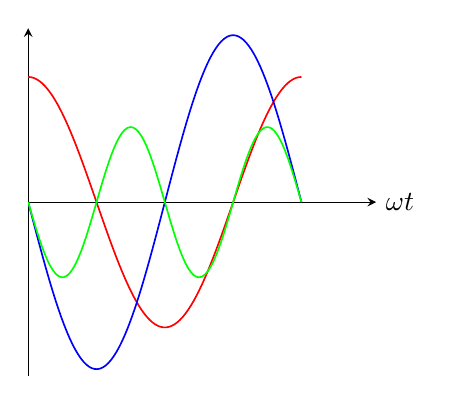
\begin{tikzpicture}
\begin{axis}[
    width=6cm, 
    height=6cm,
    axis x line=center, 
    axis y line=middle, 
    xlabel={$\omega t$},
     x label style={at={(current axis.right of origin)}, right},
    samples=100,
    ymin=-1.25, ymax=1.25,
    xmin=0, xmax=8,
    domain=0.0*pi:2*pi,
    ticks=none
]
\addplot [mark=none, semithick, red] {0.9*cos(deg(x))};
\addplot [mark=none, semithick, blue] {-1.2*sin(deg(x))};
\addplot [mark=none, semithick, green] {-1.2*sin(deg(x))*0.9*cos(deg(x))};
\end{axis}
\end{tikzpicture}  
